% Provenance (never printed): see sources/outline_sources.md (Year 3: gravitational
% potential, spherical harmonics, J2, reference ellipsoid, geoid, satellite gravimetry,
% flexure of the lithosphere). Brief: sources/book5/BRIEFS.md, ch. 3. Curves from
% figdata/bachelor-3/hydrostatic_figure.py, ice_mass.py (IMBIE 2021), flexure.py.
% Exercise and problem values in the Book 5 scratch calculator calc/ch03.py.
\chapter{Pesanteur et forme de la Terre}\label{ch:b3:gravity-geodesy}

Deux satellites se suivent autour de la Terre, l'un derrière l'autre, à une altitude
supérieure à \qty{500}{km} et distants d'environ \qty{220}{km}, et mesurent en permanence la distance
qui les sépare, à mieux qu'un micromètre près.
% ledger: geod5:grace, geod5:grace-ranging
Lorsqu'ils survolent une région où la masse est concentrée, le satellite de tête est attiré
en premier et l'écart s'accroît~; le satellite qui suit est ensuite attiré à son tour et
l'écart se réduit. À partir de ces variations infimes, mois après mois depuis 2002, on a
cartographié le champ de pesanteur terrestre et son évolution~: l'eau stockée dans les bassins
fluviaux monte et descend au rythme des saisons, tandis que les grandes calottes glaciaires
du Groenland et de l'Antarctique perdent de la masse d'année en année. La pesanteur pèse
ce que l'œil ne voit pas. Ce chapitre construit le champ de pesanteur d'une planète en
rotation à partir de son potentiel, en déduit l'aplatissement et le moment d'inertie, suit
ses anomalies jusqu'en orbite, puis s'intéresse à l'un des phénomènes que la pesanteur révèle
en surface~: la flexion de la lithosphère sous le poids d'un volcan.

\begin{recall}
La loi de la gravitation de Newton, l'énergie potentielle de gravitation et la force
centrifuge dans un référentiel tournant sont traitées dans les volumes de physique~; les moments
d'inertie d'un solide et les polynômes de Legendre $P_2(x) = (3x^2 - 1)/2$ figurent dans les
volumes universitaires de physique et de mathématiques, le module d'Young $E$ et le coefficient
de Poisson $\nu$ dans le volume de physique de troisième année. La géodésie et l'aplatissement
$f = (a - b)/a$ d'un ellipsoïde de demi-axes $a > b$ ont été rencontrés en
année~10. L'isostasie, la compensation d'Airy, la pesanteur normale, le géoïde,
la hauteur du géoïde et les anomalies de pesanteur ont été définis dans le volume de première année, dans son
chapitre sur l'isostasie et les anomalies de pesanteur.
\end{recall}

\section{Le géopotentiel}

Sur une planète en rotation, un corps au repos subit l'attraction de la masse de la planète et,
dans le référentiel qui tourne avec elle, la force centrifuge. Ces deux forces dérivent d'un
potentiel.

\begin{definition}[Géopotentiel]\label{def:b3:gravity-geodesy:geopotential}
Le \emph{géopotentiel}\index{géopotentiel} est l'énergie potentielle par unité de masse,
dans le référentiel lié à la Terre qui tourne à la vitesse angulaire $\omega$, de la gravitation
et de la force centrifuge réunies~:
\[
  W(\mathbf r) = V(\mathbf r) + \Phi(\mathbf r),\qquad
  V(\mathbf r) = -G\int_{\text{Terre}}\frac{\mathrm dm'}{|\mathbf r - \mathbf r'|},\qquad
  \Phi(\mathbf r) = -\tfrac12\omega^2 s^2,
\]
où $s$ désigne la distance à l'axe de rotation. La pesanteur vaut
$\mathbf g = -\nabla W$, et les surfaces $W = \text{cste}$ en sont les surfaces
d'égal potentiel~: la pesanteur leur est partout normale.
\end{definition}

Un fil à plomb s'aligne sur $-\nabla W$, et l'eau tranquille prend la forme d'une surface
d'égal potentiel. Une planète fluide en rotation adopte donc la forme de l'une de ses propres
surfaces d'égal potentiel~: le potentiel centrifuge, maximal à l'équateur, gonfle l'équateur
et aplatit les pôles.

\begin{omfigure}
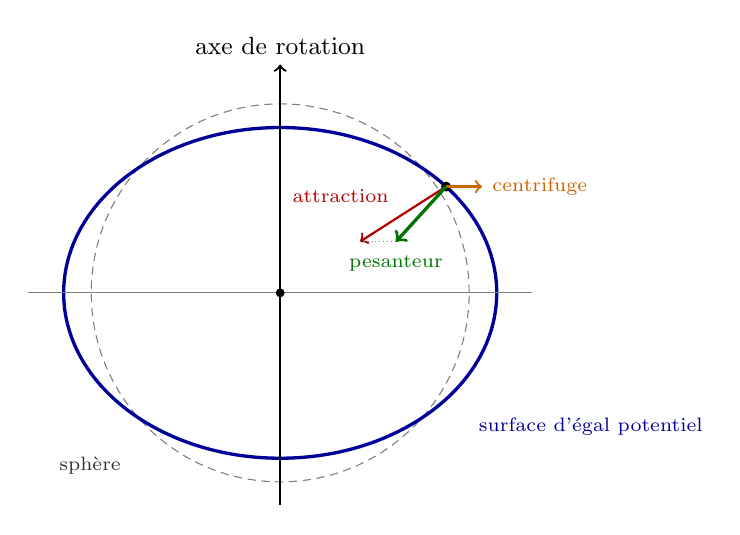
\begin{tikzpicture}[font=\small, x=1cm, y=1cm]
\draw[gray, densely dashed] (0,0) circle (2.4);
\draw[very thick, blue!60!black] (0,0) ellipse (2.75 and 2.1);
\draw[->, thick] (0,-2.7) -- (0,2.9) node[above] {axe de rotation};
\draw[gray] (-3.2,0) -- (3.2,0);
\fill (0,0) circle (1.6pt);
% a point at latitude 40 deg (parameter) on the ellipse; the attraction points at
% the centre, the centrifugal force is horizontal, and their sum is drawn along the
% inward normal of the ellipse: lengths solved so that the sum is normal (calc/ch03_fig.py)
\coordinate (P) at (2.107,1.350);
\fill (P) circle (1.8pt);
\draw[->, thick, red!70!black] (P) -- (1.012,0.650);
\node[font=\scriptsize, red!70!black, anchor=south east] at (1.50,1.02) {attraction};
\draw[->, thick, orange!80!black] (P) -- (2.565,1.350) node[right, font=\scriptsize] {centrifuge};
\draw[gray, densely dotted] (1.012,0.650) -- (1.470,0.650);
\draw[->, very thick, green!45!black] (P) -- (1.470,0.650);
\node[font=\scriptsize, green!45!black, anchor=north] at (1.470,0.600) {pesanteur};
\node[blue!60!black, anchor=west, font=\scriptsize] at (2.4,-1.7) {surface d'égal potentiel};
\node[gray!40!black, anchor=east, font=\scriptsize] at (-1.9,-2.2) {sphère};
\end{tikzpicture}

\par\smallskip{\small Une surface d'égal potentiel d'une planète en rotation (schéma,
aplatissement fortement exagéré). En chaque point, la pesanteur, somme de l'attraction et de la
force centrifuge, est normale à cette surface~; elle ne
pointe vers le centre qu'aux pôles et à l'équateur.}
\label{fig:b3:gravity-geodesy:equipotential}
\end{omfigure}

À l'extérieur de la planète, le potentiel gravitationnel vérifie l'équation de Laplace, et ses
solutions régulières à l'infini sont les harmoniques sphériques solides.

\begin{proposition}[Développement en harmoniques sphériques du géopotentiel]\label{prop:b3:gravity-geodesy:harmonics}
À l'extérieur d'un corps de masse $M$ et de rayon équatorial $a$, l'origine étant placée en son
centre de masse et l'axe $z$ suivant son axe de rotation, le potentiel gravitationnel à la
distance $r$, à la colatitude $\theta$ et à la longitude $\lambda$ vaut
\begin{multline*}
  V = -\frac{GM}{r}\Biggl[1 - \sum_{n=2}^{\infty}\left(\frac ar\right)^nJ_nP_n(\cos\theta)\\
  + \sum_{n=2}^{\infty}\sum_{m=1}^{n}\left(\frac ar\right)^nP_{nm}(\cos\theta)
  (C_{nm}\cos m\lambda + S_{nm}\sin m\lambda)\Biggr],
\end{multline*}
avec les polynômes de Legendre $P_n$ et les fonctions associées $P_{nm}$~; les coefficients
$J_n$, $C_{nm}$, $S_{nm}$ sont des nombres, ajustés sur les observations. Pour un corps à symétrie
de révolution autour de son axe, seuls les termes zonaux $J_n$ subsistent. Aucun terme de degré 1
n'apparaît.
\end{proposition}

\begin{proof}
La séparation des variables de l'équation de Laplace en coordonnées sphériques
donne les solutions régulières à l'infini $r^{-(n+1)}P_{nm}(\cos\theta)e^{\pm
im\lambda}$ (volumes universitaires de mathématiques)~; tout potentiel à l'extérieur
des masses en est une somme. Le terme de degré 0 vaut $-GM/r$, potentiel de
la masse totale. Les termes de degré 1 sont proportionnels aux moments
premiers $\int\mathbf r'\,\mathrm dm'$, qui s'annulent lorsque l'origine est le centre de
masse. La symétrie axiale supprime tout terme dépendant de $\lambda$.
\end{proof}

\begin{definition}[Facteur de forme dynamique]\label{def:b3:gravity-geodesy:j2}
Le \emph{facteur de forme dynamique}\index{facteur de forme dynamique} $J_2$ d'une planète
est le coefficient de son harmonique zonale de degré 2~: l'écart maximal de son
potentiel extérieur par rapport à celui d'une sphère, causé par son aplatissement. Pour la
Terre, $J_2 = \num{1.08263e-3}$.
% ledger: geod5:grs80-defining
\end{definition}

\begin{theorem}[Formule de MacCullagh]\label{thm:b3:gravity-geodesy:maccullagh}
Soient $A$, $B$, $C$ les moments d'inertie principaux d'un corps de masse $M$
par rapport à des axes passant par son centre de masse, et $I$ son moment d'inertie par rapport à la
droite joignant le centre de masse à un point extérieur situé à la distance $r$. À l'ordre
$r^{-3}$, le potentiel gravitationnel en ce point est donné par la
\emph{formule de MacCullagh}\index{formule de MacCullagh}
\[
  V = -\frac{GM}{r} - \frac{G(A + B + C - 3I)}{2r^3} .
\]
Pour un corps symétrique par rapport à l'axe $z$ ($A = B$),
$V = -\dfrac{GM}{r} + \dfrac{G(C - A)}{r^3}P_2(\cos\theta)$, d'où
\[
  J_2 = \frac{C - A}{Ma^2} .
\]
\end{theorem}

\begin{proof}
Avec $\hat{\mathbf r}$ le vecteur unitaire dirigé vers le point et $r' \ll r$,
\[
  \frac{1}{|\mathbf r - \mathbf r'|} = \frac1r + \frac{\hat{\mathbf r}\cdot\mathbf r'}{r^2}
  + \frac{3(\hat{\mathbf r}\cdot\mathbf r')^2 - r'^2}{2r^3} + O(r^{-4}).
\]
Intégré sur la masse, le premier terme donne $M/r$ et le second s'annule
(centre de masse). Pour le troisième, $\int r'^2\,\mathrm dm' = (A + B + C)/2$, puisque
$A + B + C = \int 2r'^2\,\mathrm dm'$, et $\int(\hat{\mathbf r}\cdot\mathbf
r')^2\,\mathrm dm' = \int r'^2\,\mathrm dm' - I$, le carré de la distance à
la droite étant $r'^2 - (\hat{\mathbf r}\cdot\mathbf r')^2$. Le crochet s'intègre
en $3(A + B + C)/2 - 3I - (A + B + C)/2 = A + B + C - 3I$. Pour $A = B$, le
moment par rapport à une droite de colatitude $\theta$ vaut $I = A\sin^2\theta + C\cos^2\theta$,
et $2A + C - 3I = (C - A)(1 - 3\cos^2\theta) = -2(C - A)P_2(\cos\theta)$.
En comparant avec la \cref{prop:b3:gravity-geodesy:harmonics}, on obtient
$J_2Ma^2 = C - A$.
\end{proof}

Le terme de degré 2 du potentiel mesure donc la différence des
moments d'inertie, et non les moments eux-mêmes. La précession de l'axe de la
Terre, provoquée par les couples exercés par le Soleil et la Lune sur le renflement
équatorial, mesure l'ellipticité dynamique $H = (C - A)/C$~; ensemble, $J_2$ et $H$ donnent
$C/(Ma^2)$, le facteur de moment d'inertie, \num{0.3308} pour la Terre,
% ledger: earth:MoI
bien en dessous des \num{0.4} d'une sphère homogène~: la masse est concentrée vers
le centre.

\section{L'ellipsoïde en rotation}

\begin{definition}[Ellipsoïde de référence]\label{def:b3:gravity-geodesy:ellipsoid}
Un \emph{ellipsoïde de référence}\index{ellipsoïde de référence} est un ellipsoïde de
révolution, de demi-axe équatorial $a$ et d'aplatissement $f$, choisi de sorte qu'il
soit lui-même une surface équipotentielle d'un potentiel modèle~: le potentiel d'un
corps en rotation de masse $M$, de vitesse angulaire $\omega$ et de \omterm{def:b3:gravity-geodesy:j2}{facteur de forme
dynamique} $J_2$ de la Terre. Quatre constantes le définissent~; le Geodetic Reference
System 1980 retient
\begin{gather*}
  a = \qty{6378137}{m},\qquad GM = \qty{3.986005e14}{m^3.s^{-2}},\\
  J_2 = \num{1.08263e-3},\qquad \omega = \qty{7.292115e-5}{rad.s^{-1}},
\end{gather*}
et en déduit l'aplatissement $f = \num{0.00335281068}$
($1/f = \num{298.257222}$) ainsi que le demi-petit axe
$b = \qty{6356752.3141}{m}$.
% ledger: geod5:grs80-defining, geod5:grs80-derived
\end{definition}

Le potentiel du modèle, le potentiel normal, est connu sous forme fermée, et il en va de même de
sa pesanteur sur l'ellipsoïde, la pesanteur normale du volume de première année.

\begin{proposition}[Formule de Somigliana]\label{prop:b3:gravity-geodesy:somigliana}
Sur un \omterm{def:b3:gravity-geodesy:ellipsoid}{ellipsoïde de référence} de demi-axes $a$, $b$ et de pesanteur normale
$\gamma_e$ à l'équateur et $\gamma_p$ aux pôles, la pesanteur normale à la
latitude géodésique $\varphi$ est donnée par la \emph{formule de
Somigliana}\index{formule de Somigliana}
\[
  \gamma(\varphi) = \frac{a\gamma_e\cos^2\varphi + b\gamma_p\sin^2\varphi}
  {\sqrt{a^2\cos^2\varphi + b^2\sin^2\varphi}} .
\]
Pour le Geodetic Reference System 1980, $\gamma_e = \qty{9.7803267715}{m.s^{-2}}$
et $\gamma_p = \qty{9.8321863685}{m.s^{-2}}$, et la série
$\gamma = 9.780327(1 + 0.0053024\sin^2\varphi - 0.0000058\sin^22\varphi)$
\unit{m.s^{-2}} reproduit la formule à \qty{0.1}{\milli\gal}~près.
% ledger: geod5:grs80-derived, moritz:grs80 (Book 3, read-only)
\end{proposition}
\admitted

Quelle doit être l'aplatissement d'une planète en rotation~? Si c'est un fluide en
équilibre hydrostatique, son aplatissement est fixé par sa rotation et par la façon dont sa masse
est répartie en profondeur.

\begin{proposition}[Relations de Clairaut et de Darwin--Radau]\label{prop:b3:gravity-geodesy:clairaut}
Pour une planète en équilibre hydrostatique, avec $m = \omega^2a^2b/(GM)$ le rapport
de l'accélération centrifuge à l'accélération gravitationnelle à l'équateur, au premier
ordre en $f$ et $m$~:
\[
  J_2 = \frac{2f - m}{3}\qquad\text{(Clairaut)},\qquad
  \frac{C}{Ma^2} = \frac23\left[1 - \frac25\sqrt{\frac52\frac mf - 1}\right]
  \qquad\text{(Darwin--Radau)} .
\]
Une planète homogène ($C/Ma^2 = 0.4$) a $f = 5m/4$~; une planète dont la masse est
concentrée vers le centre est moins aplatie.
\end{proposition}
\admitted

La relation de Clairaut, avec le $m = \num{0.00344979}$ de la Terre, transforme son
$J_2$ mesuré en $f = \num{0.0033488}$, soit $1/298.6$~: à
\qty{0.12}{\percent} près de l'aplatissement de l'ellipsoïde. La relation de Darwin--Radau,
avec le facteur de moment d'inertie, donne l'aplatissement que la Terre aurait
si c'était un fluide en équilibre~: $1/299.9$, contre
$1/298.26$ mesuré. La Terre est un peu plus aplatie qu'une planète fluide ayant sa rotation
et une répartition de masse donnée~: son renflement équatorial dépasse d'environ
\qty{116}{m} de plus que ce que prévoit l'équilibre hydrostatique. La Terre n'est pas
exactement un fluide en équilibre, et l'écart est lui-même une
mesure des contraintes que supporte son intérieur.

\begin{omfigure}
\begin{tikzpicture}
\begin{axis}[omrecord, width=0.74\linewidth, height=0.44\linewidth,
  xmin=0.3, xmax=0.4, ymin=225, ymax=340,
  xlabel={facteur de moment d'inertie $C/(Ma^2)$}, ylabel={$1/f$ hydrostatique},
  xtick={0.30,0.32,0.34,0.36,0.38,0.40},
  xticklabel style={/pgf/number format/fixed, /pgf/number format/precision=2}]
\addplot[blue!70!black, thick] table[x=moi, y=f_inv] {figdata/out/bachelor-3-hydrostatic_figure-curve.dat};
\draw[gray, densely dashed] (axis cs:0.3308,225) -- (axis cs:0.3308,299.88);
\draw[gray, densely dashed] (axis cs:0.3,299.88) -- (axis cs:0.3308,299.88);
\fill[blue!70!black] (axis cs:0.3308,299.88) circle (2pt);
\node[font=\scriptsize, anchor=south west] at (axis cs:0.3315,301) {Terre hydrostatique, $1/f = 299.9$};
\draw[red!70!black, thick] (axis cs:0.3,298.26) -- (axis cs:0.4,298.26);
\node[font=\scriptsize, anchor=north east, red!70!black] at (axis cs:0.399,296.5) {observée, $1/f = 298.26$};
\fill (axis cs:0.4,231.9) circle (2pt);
\node[font=\scriptsize, anchor=east] at (axis cs:0.397,233) {planète homogène};
\end{axis}
\end{tikzpicture}

\par\smallskip{\small L'aplatissement d'une planète fluide dotée de la rotation terrestre,
en fonction de son facteur de moment d'inertie, d'après la relation de Darwin--Radau
(calculé à partir du Geodetic Reference System 1980). Plus la masse est
concentrée vers le centre, plus la planète est ronde. Pour la valeur terrestre de
\num{0.3308} l'aplatissement hydrostatique vaut $1/299.9$, un peu moins que la
valeur observée $1/298.26$.}
\label{fig:b3:gravity-geodesy:hydrostatic}
\end{omfigure}

\section{Le géoïde et le potentiel perturbateur}

Le géoïde est la surface de niveau du \omterm{def:b3:gravity-geodesy:geopotential}{géopotentiel} réel qui coïncide avec
le niveau moyen de la mer~; l'\omterm{def:b3:gravity-geodesy:ellipsoid}{ellipsoïde de référence} est une surface de niveau du
potentiel normal $U$ de même valeur, $U_0 = W_0$. Leur écart, la hauteur du
géoïde $N$, est fixé par la différence des deux potentiels.

\begin{proposition}[Formule de Bruns]\label{prop:b3:gravity-geodesy:bruns}
Soit $T = W - U$ le potentiel perturbateur. La hauteur du géoïde en un point est
donnée par la \emph{formule de Bruns}\index{formule de Bruns}
\[
  N = -\frac{T}{\gamma},
\]
où $T$ est évalué sur le géoïde et $\gamma$ est la pesanteur normale en ce point. Un
excès de masse, qui creuse le potentiel ($T < 0$), élève le géoïde.
\end{proposition}

\begin{proof}
Soit P sur le géoïde et Q le point de l'ellipsoïde situé sous lui, à la distance
$N$. Comme $U$ croît vers l'extérieur au taux $\gamma$,
$U(\mathrm P) = U(\mathrm Q) + \gamma N = U_0 + \gamma N$. Alors
$W_0 = W(\mathrm P) = U(\mathrm P) + T(\mathrm P) = U_0 + \gamma N + T$, et
$W_0 = U_0$ donne $N = -T/\gamma$.
\end{proof}

Une hauteur de géoïde de \qty{50}{m} correspond à une différence de potentiel de seulement
\qty{490}{J.kg^{-1}}, soit une partie sur \num{e5} du \omterm{def:b3:gravity-geodesy:geopotential}{géopotentiel}. Les
hauteurs du géoïde terrestre vont d'environ $+\qty{85}{m}$ en Islande à
$-\qty{106}{m}$ dans le sud de l'Inde,
% ledger: nasa:geoid-range (Book 3, read-only)
soit un écart de moins de \qty{200}{m} pour une planète dont les rayons équatorial et polaire
diffèrent de \qty{21}{km}.

\section{Gravimétrie satellitaire}

\begin{definition}[Gravimétrie satellitaire]\label{def:b3:gravity-geodesy:satgrav}
La \emph{gravimétrie satellitaire}\index{gravimétrie satellitaire} détermine le champ
de pesanteur terrestre à partir du mouvement des satellites~: perturbations à long terme
de leurs orbites, de la variation de distance entre deux satellites sur une même
orbite, ou à l'aide de gradiomètres qui mesurent les différences de pesanteur d'un bout
à l'autre de l'engin spatial.
\end{definition}

La plus grande perturbation d'une orbite proche de la Terre provient de $J_2$. Le
renflement équatorial exerce un couple sur l'orbite inclinée, qui tourne lentement
autour de l'axe terrestre.

\begin{proposition}[Précession nodale]\label{prop:b3:gravity-geodesy:nodal}
Au premier ordre en $J_2$, la ligne des nœuds d'une orbite circulaire de rayon $r$ et
d'inclinaison $i$ tourne au taux
\[
  \dot\Omega = -\frac32\,nJ_2\left(\frac ar\right)^2\cos i,\qquad n = \sqrt{GM/r^3} ,
\]
vers l'ouest pour une orbite directe ($i < \ang{90}$), vers l'est pour une orbite rétrograde.
\end{proposition}

\begin{proof}
Sur de nombreuses révolutions, le satellite se comporte comme un anneau de masse $m_s$ répartie le long
de son orbite. La partie de degré 2 du potentiel,
$(GMJ_2a^2/r^3)P_2(\cos\theta)$ par unité de masse, moyennée sur un cercle incliné
à $i$, fait intervenir $\langle\cos^2\theta\rangle = \tfrac12\sin^2i$, d'où
$\langle P_2\rangle = \tfrac34\sin^2i - \tfrac12$, et l'énergie de l'anneau vaut
$E(i) = m_s(GMJ_2a^2/r^3)(\tfrac34\sin^2i - \tfrac12)$. Le couple par rapport à la ligne
des nœuds vaut $\tau = -\mathrm dE/\mathrm di = -\tfrac32m_s(GMJ_2a^2/r^3)\sin
i\cos i$. Il est perpendiculaire au moment cinétique de l'anneau $L = m_snr^2$~: il
fait tourner $\mathbf L$ autour de l'axe polaire sans modifier sa norme~:
$L\sin i\,\dot\Omega = \tau$. Avec $GM = n^2r^3$, $\dot\Omega =
-\tfrac32nJ_2(a/r)^2\cos i$.
\end{proof}

Le taux atteint plusieurs degrés par jour pour une orbite basse proche de l'équateur~; pour une
inclinaison un peu supérieure à \ang{90}, il égale le mouvement annuel du Soleil, et l'orbite
garde la même orientation par rapport au Soleil toute l'année (exercice~12). Mesurées sur
de nombreux satellites d'inclinaisons différentes, ces précessions donnent $J_2$ et les
harmoniques zonales d'ordre supérieur.

Une paire de satellites fait mieux~: la variation de distance entre eux mesure la
différence de pesanteur ressentie le long de l'orbite. Le couple GRACE a fonctionné de 2002 à 2017, et son
successeur, GRACE Follow-On, depuis son lancement le \num{22}~mai 2018, sa liaison micro-onde
mesurant la distance à mieux d'un micromètre près, et une liaison laser en test visant une
précision jusqu'à vingt fois meilleure.
% ledger: geod5:grace, geod5:grace-ranging
Le champ varie d'un mois à l'autre parce que l'eau se déplace~: neige et humidité
des sols, eaux souterraines, lacs, océans, calottes glaciaires.

\begin{omfigure}
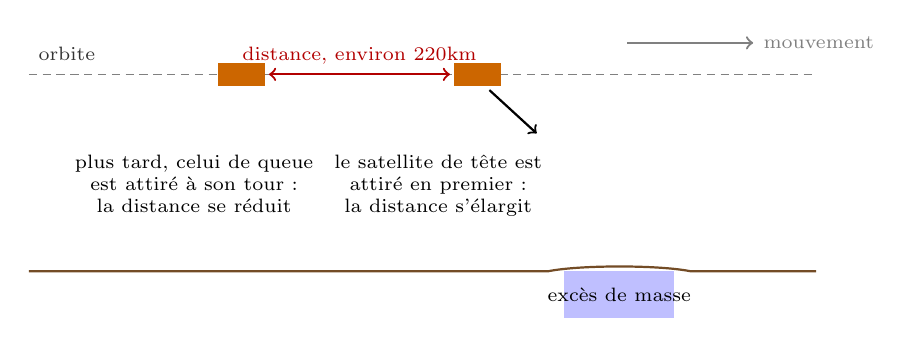
\begin{tikzpicture}[font=\small, x=1cm, y=1cm]
\draw[thick, brown!60!black] (-5,0) -- (1.6,0) .. controls (2.0,0.08) and (3.0,0.08) .. (3.4,0) -- (5,0);
\fill[blue!25] (1.8,0) rectangle (3.2,-0.6);
\node[font=\scriptsize] at (2.5,-0.3) {excès de masse};
\draw[gray, densely dashed] (-5,2.5) -- (5,2.5);
\node[gray!40!black, font=\scriptsize, anchor=south west] at (-5,2.55) {orbite};
\fill[orange!80!black] (-2.6,2.35) rectangle (-2.0,2.65);
\fill[orange!80!black] (0.4,2.35) rectangle (1.0,2.65);
\draw[<->, red!70!black, thick] (-1.95,2.5) -- (0.35,2.5) node[midway, above, font=\scriptsize] {distance, environ \qty{220}{km}};
\draw[->, thick] (0.85,2.3) -- (1.45,1.75);
\draw[->, thick, gray] (2.6,2.9) -- (4.2,2.9) node[right, font=\scriptsize] {mouvement};
\node[font=\scriptsize, anchor=north, align=center] at (0.2,1.6) {le satellite de tête est\\attiré en premier~:\\la distance s'élargit};
\node[font=\scriptsize, anchor=north, align=center] at (-2.9,1.6) {plus tard, celui de queue\\est attiré à son tour~:\\la distance se réduit};
\end{tikzpicture}

\par\smallskip{\small Le principe de la paire de satellites (schématique, non à
l'échelle). À l'approche d'un excès de masse, le satellite de tête en ressent
d'abord l'attraction et est accéléré vers l'avant, si bien que la distance entre
les deux augmente~; lorsque le satellite de queue passe au-dessus de la masse, la
distance diminue à nouveau. La vitesse relative, mesurée en continu, est inversée pour obtenir le champ de pesanteur.}
\label{fig:b3:gravity-geodesy:grace}
\end{omfigure}

\begin{omfigure}
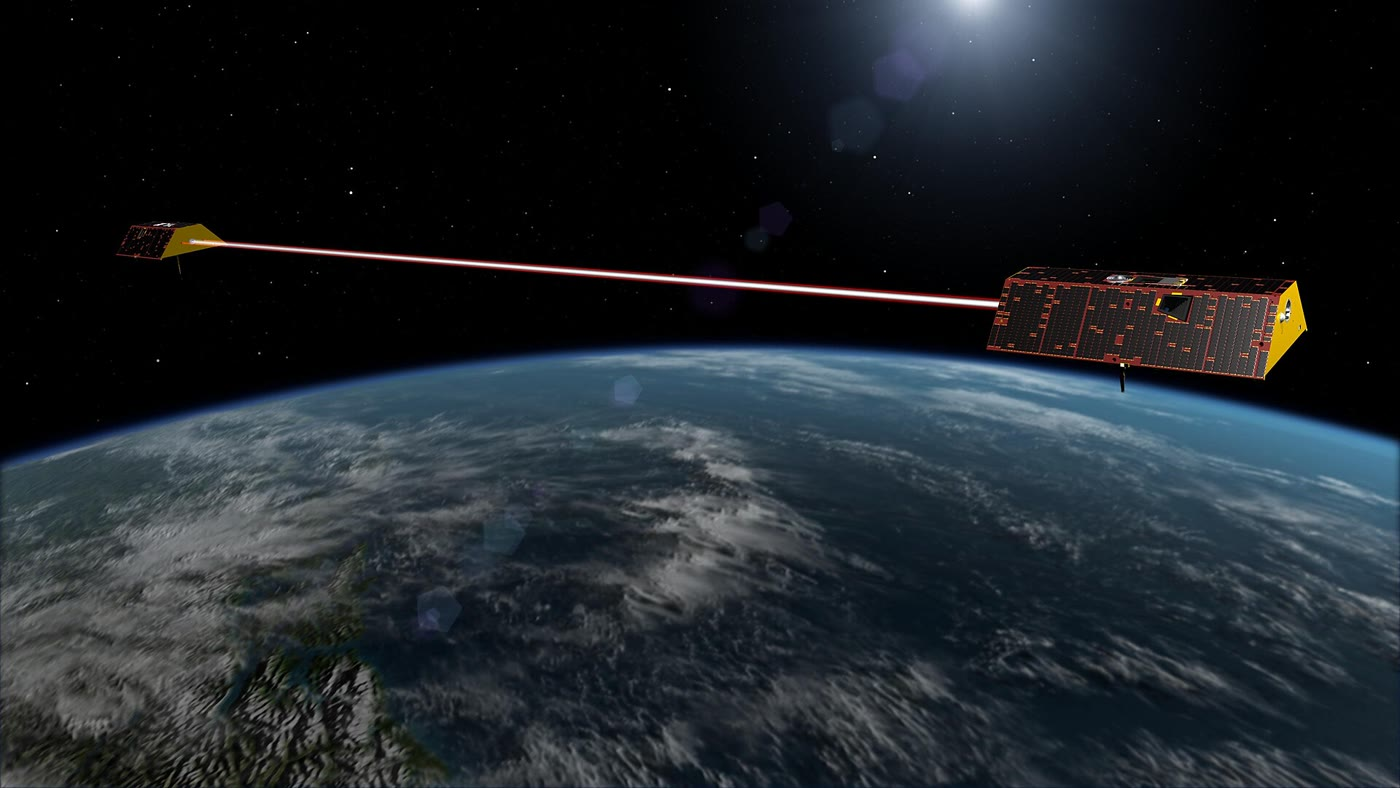
\includegraphics[width=0.66\linewidth]{images/book5/b3-grace-fo-concept.jpg}

\par\smallskip{\small Les deux satellites GRACE Follow-On, vue d'artiste (la
distance entre eux est fortement réduite). Le faisceau rouge représente la
liaison laser de mesure de distance. NASA/JPL-Caltech, domaine public.}
\label{fig:b3:gravity-geodesy:grace-photo}
\end{omfigure}

\begin{definition}[Hauteur d'eau équivalente]\label{def:b3:gravity-geodesy:ewh}
Une variation du champ de pesanteur qui varie lentement sur des distances bien
supérieures à l'épaisseur de la couche où la masse s'est déplacée peut être
représentée par une variation de densité surfacique $\sigma$ (\unit{kg.m^{-2}})
sur une coque mince à la surface de la Terre. La \emph{hauteur d'eau équivalente}\index{hauteur d'eau équivalente}
est l'épaisseur d'eau douce ayant la même densité surfacique~:
\[
  h_w = \frac{\sigma}{\rho_w} .
\]
\end{definition}

Un mètre d'eau sur un bassin de \qty{1e6}{km^2} représente \qty{1e15}{kg}, soit
\qty{1000}{Gt}. Le niveau de la mer est l'autre face du bilan~: \qty{360}{Gt} de glace
ajoutée à l'océan le relève d'environ un millimètre.
% ledger: data:b5-imbie
La \omterm{def:b3:gravity-geodesy:satgrav}{gravimétrie satellitaire}, l'altimétrie satellitaire et le bilan entre
chutes de neige et débit de glace mesurent chacun le bilan de masse
des calottes glaciaires~; réconciliés, ils donnent la série ci-dessous.

\begin{omfigure}
\begin{tikzpicture}
\begin{axis}[omrecord, width=0.82\linewidth, height=0.5\linewidth,
  xmin=1992, xmax=2021, ymin=-5600, ymax=600,
  xlabel={année}, ylabel={variation de masse cumulée (\unit{Gt})},
  xticklabel style={/pgf/number format/1000 sep={}},
  legend pos=south west, legend cell align=left, legend style={font=\scriptsize}]
\addplot[name path=gl, draw=none, forget plot] table[x=year, y=lo] {figdata/out/bachelor-3-ice_mass-greenland.dat};
\addplot[name path=gh, draw=none, forget plot] table[x=year, y=hi] {figdata/out/bachelor-3-ice_mass-greenland.dat};
\addplot[blue!25, forget plot] fill between[of=gl and gh];
\addplot[name path=al, draw=none, forget plot] table[x=year, y=lo] {figdata/out/bachelor-3-ice_mass-antarctica.dat};
\addplot[name path=ah, draw=none, forget plot] table[x=year, y=hi] {figdata/out/bachelor-3-ice_mass-antarctica.dat};
\addplot[red!20, forget plot] fill between[of=al and ah];
\addplot[blue!70!black, thick] table[x=year, y=cum] {figdata/out/bachelor-3-ice_mass-greenland.dat};
\addlegendentry{Groenland}
\addplot[red!70!black, thick] table[x=year, y=cum] {figdata/out/bachelor-3-ice_mass-antarctica.dat};
\addlegendentry{Antarctique}
\draw[gray, densely dotted] (axis cs:2002.25,-5600) -- (axis cs:2002.25,600);
\draw[gray, densely dotted] (axis cs:2017.5,-5600) -- (axis cs:2017.5,600);
\node[font=\scriptsize, gray!40!black, anchor=north] at (axis cs:2009.9,550) {années GRACE};
\end{axis}
\end{tikzpicture}

\par\smallskip{\small Variation de masse cumulée des calottes glaciaires du Groenland et de l'Antarctique
depuis 1992, avec des bandes d'un écart type (estimations réconciliées IMBIE 2021
issues de l'altimétrie, de la gravimétrie et de la méthode entrée--sortie). À la fin
de 2020, le Groenland avait perdu $\num{4890} \pm \qty{460}{Gt}$ et l'Antarctique
$\num{2670} \pm \qty{530}{Gt}$~; les ajustements linéaires donnent
\qty{-176}{Gt.an^{-1}} et \qty{-91}{Gt.an^{-1}} sur 1992--2020, et
\qty{-246}{Gt.an^{-1}} et \qty{-127}{Gt.an^{-1}} sur les années GRACE.}
\label{fig:b3:gravity-geodesy:ice-mass}
\end{omfigure}

Une anomalie de pesanteur mesurée à la surface est une somme d'harmoniques~; à
la hauteur d'un satellite, chacune est affaiblie par un facteur qui dépend de sa
longueur d'onde.

\begin{proposition}[Prolongement vers le haut]\label{prop:b3:gravity-geodesy:upward}
Au-dessus des masses qui la causent, une anomalie de pesanteur qui varie le long
de la surface comme $\Delta g_0\cos kx$, avec $k = 2\pi/\lambda$, vaut à la
hauteur $z$ (son \emph{prolongement vers le haut}\index{prolongement vers le haut})
\[
  \Delta g(x, z) = \Delta g_0\,e^{-kz}\cos kx .
\]
\end{proposition}

\begin{proof}
Au-dessus des masses, le potentiel anormal, et avec lui l'anomalie, vérifie
l'équation de Laplace $\partial_x^2\Delta g + \partial_z^2\Delta g = 0$. En
séparant les variables, $\Delta g = Z(z)\cos kx$ avec $Z'' = k^2Z$, dont la
solution bornée lorsque $z \to \infty$ est $Z = \Delta g_0e^{-kz}$.
\end{proof}

À une hauteur de \qty{400}{km}, une anomalie longue de \qty{1000}{km} conserve \qty{8}{\percent}
de son amplitude, une anomalie de \qty{100}{km} n'en conserve qu'environ \num{1e-11}~:
les satellites voient les grandes longueurs d'onde, et les mesures en surface les courtes.

\section{Flexure lithosphérique}

Le volume de première année compensait une charge localement, chaque colonne flottant pour son propre compte.
Un volcan posé sur une plaque océanique n'est pas compensé sous lui seul~: la
plaque fléchit sous lui sur une largeur de plusieurs centaines de kilomètres, et le fond marin
autour du volcan s'enfonce dans une fosse, au-delà de laquelle il remonte en un arc bas.

\begin{definition}[Flexure lithosphérique, rigidité flexurale, épaisseur élastique effective]\label{def:b3:gravity-geodesy:flexure}
\emph{flexure lithosphérique}\index{flexure lithosphérique} est le fléchissement de la
lithosphère sous une charge, modélisé comme le fléchissement d'une plaque élastique mince. La
résistance de la plaque au fléchissement est sa
\emph{rigidité flexurale}\index{rigidité flexurale}
\[
  D = \frac{ET_e^3}{12(1 - \nu^2)},
\]
et l'épaisseur $T_e$ de la plaque élastique uniforme qui fléchit comme la
lithosphère réelle est son \emph{épaisseur élastique effective}\index{epaisseur élastique effective@épaisseur élastique effective}.
\end{definition}

\begin{theorem}[Flexure d'une plaque mince]\label{thm:b3:gravity-geodesy:plate}
Une plaque élastique mince de rigidité $D$, fléchie dans une direction par une charge $q(x)$
par unité de surface, fléchie vers le bas d'une quantité $w(x)$ et flottant sur un manteau de masse volumique
$\rho_m$, le creux étant comblé par un matériau de masse volumique $\rho_i$, obéit
à l'\emph{équation de la flexure}\index{equation de la flexure@équation de la flexure}
\[
  D\frac{\mathrm d^4w}{\mathrm dx^4} + (\rho_m - \rho_i)g\,w = q(x) .
\]
\end{theorem}

\begin{proof}
Dans une plaque fléchie, les fibres situées au-dessus du plan médian sont raccourcies et celles au-dessous
allongées, proportionnellement à la courbure $w''$~; en intégrant la contrainte de
flexion sur l'épaisseur donne le moment fléchissant $M = -Dw''$, avec la
rigidité de la définition (la plaque ne peut pas se dilater latéralement, d'où le facteur
$1 - \nu^2$~; le volume de troisième année des volumes de physique). Une tranche $\mathrm dx$ de la plaque
porte l'effort tranchant $V$ sur ses faces et le moment $M$. Équilibre vertical~:
la charge $q\,\mathrm dx$ vers le bas et la poussée d'Archimède du manteau déplacé
$(\rho_m - \rho_i)gw\,\mathrm dx$ vers le haut donnent $\mathrm dV/\mathrm dx = -q +
(\rho_m - \rho_i)gw$. L'équilibre des moments donne $\mathrm dM/\mathrm dx = V$.
Alors $-Dw'''' = M'' = V' = -q + (\rho_m - \rho_i)gw$.
\end{proof}

\begin{definition}[Paramètre flexural, bombement périphérique]\label{def:b3:gravity-geodesy:alpha}
Le \emph{paramètre flexural}\index{paramètre flexural} d'une plaque est la
longueur
\[
  \alpha = \left(\frac{4D}{(\rho_m - \rho_i)g}\right)^{1/4},
\]
qui fixe l'échelle horizontale de sa flexure. Le \emph{bombement périphérique}\index{bombement périphérique}
est le faible arc de flexure vers le haut que soulève une plaque fléchie au-delà de la fosse ou
bassin voisin de sa charge.
\end{definition}

\begin{proposition}[Charge linéique sur une plaque continue]\label{prop:b3:gravity-geodesy:line}
Une charge linéique $V_0$ par unité de longueur le long de $x = 0$ fléchit la plaque de
\[
  w(x) = w_0e^{-|x|/\alpha}\left(\cos\frac{|x|}{\alpha} + \sin\frac{|x|}{\alpha}\right),
  \qquad w_0 = \frac{V_0\alpha^3}{8D} .
\]
  La flèche s'annule en $|x| = 3\pi\alpha/4$, au bord de la fosse~; la
crête du \omterm{def:b3:gravity-geodesy:alpha}{bombement périphérique} est en $|x| = \pi\alpha$, avec la hauteur $w_0e^{-\pi} =
\num{0.0432}\,w_0$. La poussée d'Archimède de l'ensemble de la flèche équilibre la charge~:
$\int(\rho_m - \rho_i)gw\,\mathrm dx = V_0$.
\end{proposition}

\begin{proof}
Pour $x > 0$ l'équation s'écrit $w'''' + 4w/\alpha^4 = 0$~; les racines de
$r^4 = -4/\alpha^4$ sont $(\pm1 \pm i)/\alpha$, et les solutions qui s'annulent à
l'infini sont $e^{-x/\alpha}(A\cos(x/\alpha) + B\sin(x/\alpha))$. La symétrie impose
$w'(0) = 0$, ce qui donne $A = B = w_0$. En intégrant l'équilibre vertical à travers
la charge, l'effort tranchant $V = -Dw'''$ subit un saut de $-V_0$~; par symétrie
$w'''(0^-) = -w'''(0^+)$, et $w'''(0^+) = 4w_0/\alpha^3$, donc $8Dw_0/\alpha^3 =
V_0$. La flèche s'annule là où $\tan(x/\alpha) =
-1$, d'abord en $x = 3\pi\alpha/4$~; sa dérivée,
$-(2w_0/\alpha)e^{-x/\alpha}\sin(x/\alpha)$, s'annule ensuite en $x = \pi\alpha$.
Enfin $\int_0^\infty e^{-u}(\cos u + \sin u)\,\mathrm du = 1$, donc
$\int w\,\mathrm dx = 2w_0\alpha = V_0\alpha^4/(4D) = V_0/((\rho_m - \rho_i)g)$.
\end{proof}

\begin{proposition}[Plaque brisée]\label{prop:b3:gravity-geodesy:broken}
Une plaque brisée en $x = 0$ et enfoncée à son extrémité libre, comme au niveau d'une fosse
océanique, la plaque fléchit selon $w = w_0e^{-x/\alpha}\cos(x/\alpha)$ pour $x \ge 0$~: la
flèche s'annule en $x = \pi\alpha/2$, et la crête du \omterm{def:b3:gravity-geodesy:alpha}{bombement périphérique}, la
remontée externe, se trouve en $x = 3\pi\alpha/4$, avec une hauteur $w_0e^{-3\pi/4}/\sqrt2 =
\num{0.067}\,w_0$.
\end{proposition}

\begin{proof}
Les mêmes solutions décroissantes, avec cette fois une extrémité libre ne portant aucun moment,
$w''(0) = 0$, ce qui donne $B = 0$. Le zéro est en $\cos(x/\alpha) = 0$~; la
dérivée $-(w_0/\alpha)e^{-x/\alpha}(\cos + \sin)(x/\alpha)$ s'annule en
$x = 3\pi\alpha/4$, où $w = w_0e^{-3\pi/4}\cos(3\pi/4)$.
\end{proof}

Les distances sont donc la clé de la résistance de la plaque~: mesurer là où la fosse
se termine ou là où le bombement culmine, et $\alpha$ en découle, puis $D$, puis $T_e$.
Comme $T_e$ intervient par $\alpha^{4/3}$, une estimation correcte d'une distance donne une bonne
estimation de l'épaisseur.

\begin{omfigure}
\begin{tikzpicture}
\begin{groupplot}[group style={group size=1 by 2, vertical sep=1.5cm},
  width=0.82\linewidth, height=0.36\linewidth, xmin=-400, xmax=400,
  tick label style={font=\scriptsize}, label style={font=\small}, title style={font=\small}]
\nextgroupplot[title={(a) charge linéique~: la crête d'Oru sur des plaques de trois épaisseurs},
  ylabel={flèche (\unit{m})}, ymin=-3000, ymax=700, y filter/.expression={-y},
  legend pos=south east, legend cell align=left, legend style={font=\scriptsize}]
\addplot[red!70!black, thick] table[x=x, y=w10] {figdata/out/bachelor-3-flexure-profiles.dat};
\addlegendentry{$T_e = \qty{10}{km}$}
\addplot[blue!70!black, thick] table[x=x, y=w25] {figdata/out/bachelor-3-flexure-profiles.dat};
\addlegendentry{$T_e = \qty{25}{km}$}
\addplot[green!45!black, thick] table[x=x, y=w40] {figdata/out/bachelor-3-flexure-profiles.dat};
\addlegendentry{$T_e = \qty{40}{km}$}
\draw[gray] (axis cs:-400,0) -- (axis cs:400,0);
\draw[->, blue!70!black] (axis cs:222,330) -- (axis cs:222,90);
\node[font=\scriptsize, blue!70!black, anchor=south] at (axis cs:222,330) {bombement périphérique, $\pi\alpha$};
\nextgroupplot[title={(b) plaque brisée au niveau d'une fosse, $T_e = \qty{25}{km}$},
  xlabel={distance à la charge ou à la fosse (\unit{km})},
  ylabel={flèche (\unit{m})}, xmin=0, xmax=400, ymin=-1100, ymax=280,
  y filter/.expression={-y}]
\addplot[blue!70!black, thick] table[x=x, y=w] {figdata/out/bachelor-3-flexure-broken.dat};
\draw[gray] (axis cs:0,0) -- (axis cs:400,0);
\draw[->] (axis cs:166.5,200) -- (axis cs:166.5,80);
\node[font=\scriptsize, anchor=west] at (axis cs:170,200) {remontée externe, $3\pi\alpha/4$};
\end{groupplot}
\end{tikzpicture}

\par\smallskip{\small Flexion d'une plaque élastique (calculée~;
$E = \qty{100}{GPa}$, $\nu = 0.25$, manteau \qty{3300}{kg.m^{-3}}, eau dans la
fosse périphérique~; échelle verticale fortement exagérée). (a) Sous la charge d'une crête
volcanique (\qty{4.17e12}{N.m^{-1}}), une plaque mince s'enfonce profondément et étroitement, une plaque épaisse
peu et largement~; le \omterm{def:b3:gravity-geodesy:alpha}{bombement périphérique} s'écarte de \qty{112}{km} à
\qty{316}{km}. (b) Une plaque brisée au niveau d'une fosse et enfoncée de \qty{1}{km}~:
la remontée externe mesure \qty{67}{m} de haut, à \qty{167}{km} de la fosse.}
\label{fig:b3:gravity-geodesy:flexure}
\end{omfigure}

\begin{definition}[Compensation isostatique régionale]\label{def:b3:gravity-geodesy:regional}
\emph{compensation isostatique régionale}\index{compensation isostatique régionale}
est le soutien d'une charge par la poussée exercée par une flexion répartie sur une région
plus vaste que la charge, grâce à la résistance de la lithosphère en flexion~; en revanche, dans les compensations d'Airy
ou de Pratt, chaque colonne est compensée sous elle-même.
\end{definition}

Les compensations locale et régionale équilibrent la même masse totale, mais la répartissent
différemment~: sous une charge étroite sur une plaque rigide, la racine est peu profonde et large,
et l'anomalie de pesanteur au-dessus de la charge est fortement positive, bordée d'anomalies négatives
au-dessus de la fosse périphérique. Autour des îles de la ride hawaïenne, les profils gravimétriques et
sismiques donnent des \omterm{def:b3:gravity-geodesy:flexure}{épaisseurs élastiques effectives} de 17 à \qty{37}{km}, et
de 10 à \qty{20}{km} le long des monts sous-marins plus anciens de la chaîne d'Empereur, un écart
attendu d'après les âges des volcans et de la plaque qu'ils chargent~; les valeurs
suivent la profondeur d'une isotherme voisine de
\qty{350}{\degreeCelsius} dans la plaque océanique en refroidissement.
% ledger: watts25:te
La même flexion, sous le poids d'une chaîne de montagnes, ouvre les bassins d'avant-pays du volume de deuxième année,
dans son chapitre consacré à l'orogène alpin.

\begin{omfigure}
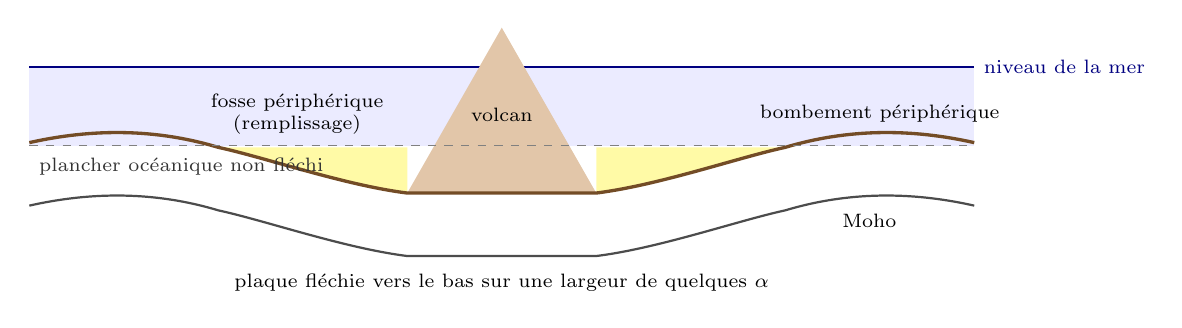
\begin{tikzpicture}[font=\scriptsize, x=1cm, y=1cm]
\fill[blue!8] (-6,0) rectangle (6,-1.0);
\draw[blue!50!black] (-6,0) -- (6,0) node[right] {niveau de la mer};
% volcano
\fill[brown!45] (-1.2,-1.6) -- (0,0.5) -- (1.2,-1.6) -- cycle;
% moat infill
\fill[yellow!35] (-1.2,-1.6) .. controls (-2.0,-1.5) and (-3.0,-1.15) .. (-3.6,-1.02) -- (-1.2,-1.02) -- cycle;
\fill[yellow!35] (1.2,-1.6) .. controls (2.0,-1.5) and (3.0,-1.15) .. (3.6,-1.02) -- (1.2,-1.02) -- cycle;
% flexed seafloor (top of crust)
\draw[very thick, brown!60!black] (-6,-0.96) .. controls (-5.2,-0.78) and (-4.4,-0.78) .. (-3.6,-1.02)
  .. controls (-3.0,-1.15) and (-2.0,-1.5) .. (-1.2,-1.6) -- (1.2,-1.6)
  .. controls (2.0,-1.5) and (3.0,-1.15) .. (3.6,-1.02) .. controls (4.4,-0.78) and (5.2,-0.78) .. (6,-0.96);
% Moho, parallel
\draw[thick, gray!60!black] (-6,-1.76) .. controls (-5.2,-1.58) and (-4.4,-1.58) .. (-3.6,-1.82)
  .. controls (-3.0,-1.95) and (-2.0,-2.3) .. (-1.2,-2.4) -- (1.2,-2.4)
  .. controls (2.0,-2.3) and (3.0,-1.95) .. (3.6,-1.82) .. controls (4.4,-1.58) and (5.2,-1.58) .. (6,-1.76);
\node[anchor=west] at (4.2,-1.95) {Moho};
\draw[dashed, gray] (-6,-1.0) -- (6,-1.0);
\node[anchor=north west, gray!40!black] at (-6,-1.03) {plancher océanique non fléchi};
\node[anchor=south, align=center] at (-2.6,-0.98) {fosse périphérique\\(remplissage)};
\node[anchor=south] at (4.8,-0.82) {bombement périphérique};
\node at (0,-0.6) {volcan};
\node[anchor=north] at (0,-2.5) {plaque fléchie vers le bas sur une largeur de quelques $\alpha$};
\end{tikzpicture}

\par\smallskip{\small Île volcanique sur une plaque océanique (coupe schématique,
échelle verticale exagérée). La plaque fléchit sous le volcan~;
la dépression qui l'entoure, la fosse périphérique, se remplit de débris volcaniques et de sédiments, et
au-delà, la plaque se soulève en un faible \omterm{def:b3:gravity-geodesy:alpha}{bombement périphérique}.}
\label{fig:b3:gravity-geodesy:moat}
\end{omfigure}

\begin{inthefield}[Un levé gravimétrique relatif]
\begin{minipage}[t]{0.55\linewidth}\vspace{0pt}
Un gravimètre absolu laisse tomber un miroir à coin de cube dans une chambre à vide, à plusieurs reprises,
et chronomètre sa chute à l'aide d'un interféromètre laser et d'une horloge atomique~;
il donne la pesanteur en une station, mais il est lourd et lent à installer. Le levé
se fait avec un gravimètre relatif, une petite balance à ressort qui mesure
les écarts de pesanteur. Le géophysicien le met à niveau sur une plaque de base à chaque
station d'un profil, le lit, note l'heure et la hauteur, puis passe à la suivante~; toutes les
quelques heures, la boucle revient à une station de base, afin de mesurer et d'éliminer la lente dérive du
ressort et les marées terrestres. Un récepteur satellitaire
posé sur un mât voisin fournit la position et la hauteur, car la pesanteur
varie d'environ \qty{0.3}{\milli\gal} pour chaque mètre de hauteur.
\end{minipage}\hfill
\begin{minipage}[t]{0.42\linewidth}\vspace{0pt}
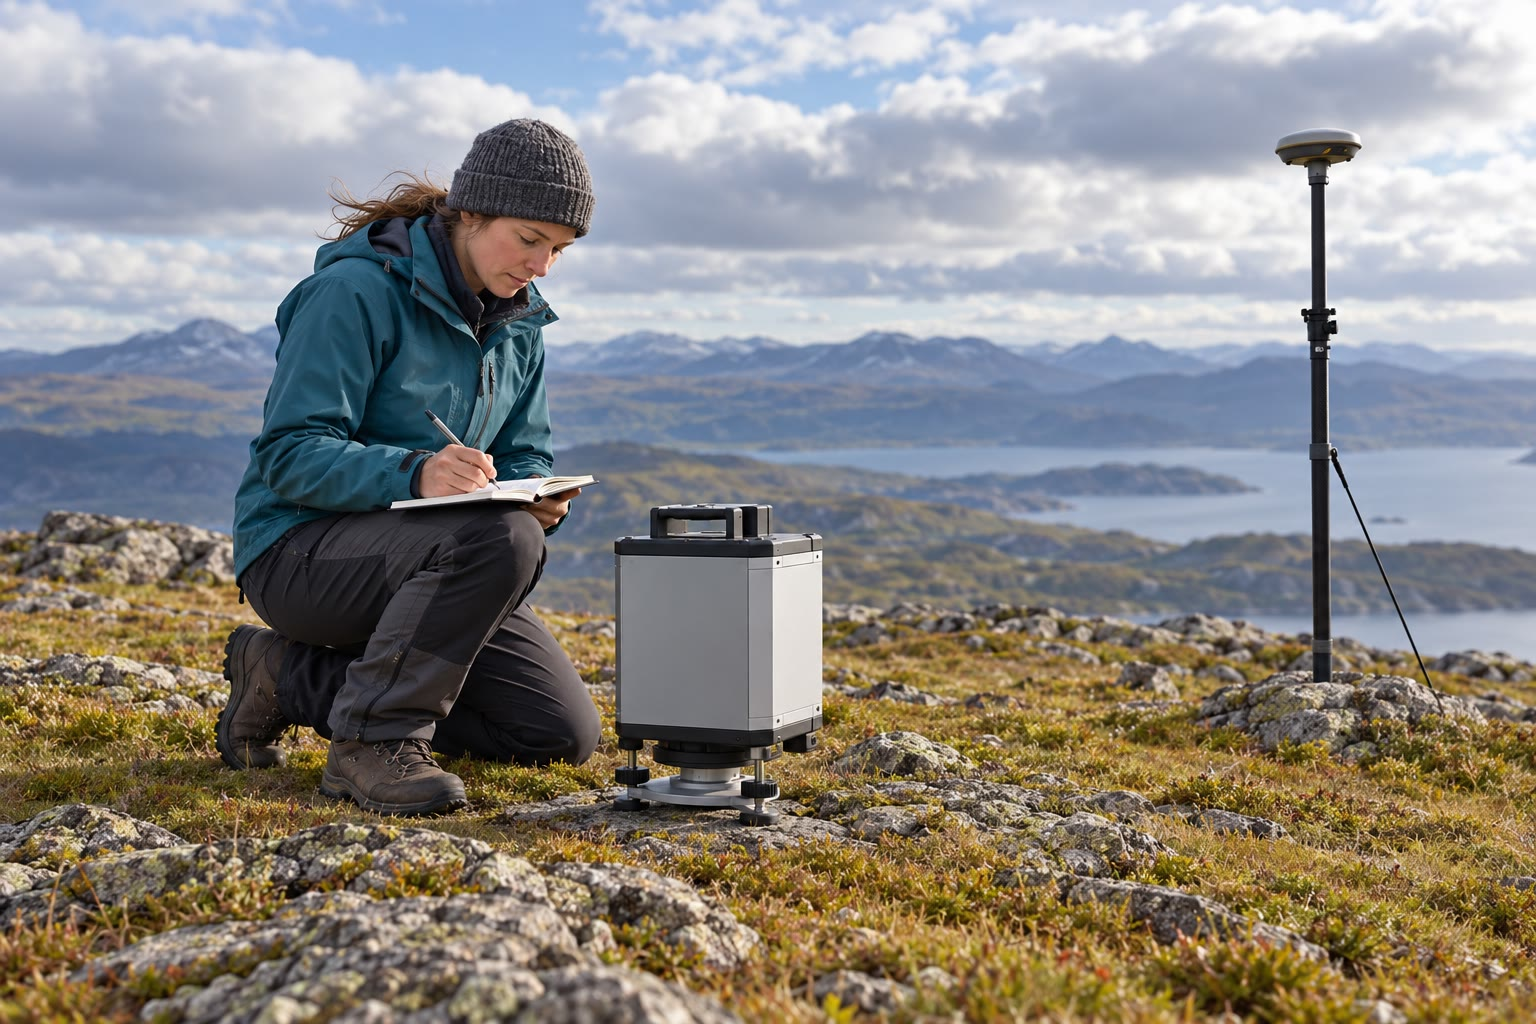
\includegraphics[width=\linewidth]{images/book5/ai/b3-gravimeter.jpg}

{\scriptsize Un gravimètre de terrain sur son socle de mise à niveau, avec une antenne satellite
en arrière-plan (Illustration générée par IA.)}
\end{minipage}
\end{inthefield}

\section{Exercices}

\begin{exercise}[$\star$]\label{exo:b3:gravity-geodesy:1}
À partir des valeurs du Geodetic Reference System 1980, $a = \qty{6378137}{m}$ et
$f = \num{0.00335281068}$, calculer le demi-petit axe $b$ et $a - b$. Avec
$J_2 = \num{1.08263e-3}$ et $m = \num{0.00344979}$, calculer l'aplatissement que
prédit la relation de Clairaut, et comparer.
\end{exercise}

\begin{exercise}[$\star$]\label{exo:b3:gravity-geodesy:2}
Une année sèche, un bassin fluvial de \qty{5.0e5}{km^2} perd \qty{60}{Gt} de
eau. Calculer la variation de \omterm{def:b3:gravity-geodesy:ewh}{hauteur d'eau équivalente}. De combien la
même masse élèverait le niveau de la mer, sachant que \qty{360}{Gt} correspondent à un millimètre~?
\end{exercise}

\begin{exercise}[$\star$]\label{exo:b3:gravity-geodesy:3}
Avec la série $\gamma = 9.780327(1 + 0.0053024\sin^2\varphi -
0.0000058\sin^22\varphi)$ \unit{m.s^{-2}}, calculer la pesanteur normale à
l'équateur, à \ang{45} et aux pôles. Exprimer la différence entre le pôle
et l'équateur en milligals.
\end{exercise}

\begin{exercise}[$\star$]\label{exo:b3:gravity-geodesy:4}
Calculer la \omterm{def:b3:gravity-geodesy:flexure}{rigidité flexurale} et le \omterm{def:b3:gravity-geodesy:alpha}{paramètre flexural} de plaques océaniques avec
$T_e = \qty{10}{km}$ et $T_e = \qty{30}{km}$ ($E = \qty{100}{GPa}$,
$\nu = 0.25$, $\rho_m - \rho_w = \qty{2270}{kg.m^{-3}}$, $g =
\qty{9.81}{m.s^{-2}}$). Où se situent le bord de la fosse périphérique et le \omterm{def:b3:gravity-geodesy:alpha}{bombement périphérique} sous une
charge linéique~?
\end{exercise}

\begin{exercise}[$\star\star$]\label{exo:b3:gravity-geodesy:5}
(a) Pour une hauteur de géoïde de $+\qty{50}{m}$~: calculer le potentiel perturbateur en ce point,
en prenant $\gamma = \qty{9.80}{m.s^{-2}}$. (b) Sur \qty{100}{km}, le géoïde s'élève
de \qty{10}{m}. De quel angle la verticale en ce point diffère-t-elle de la normale à
l'ellipsoïde~? Donner cet angle en secondes d'arc.
\end{exercise}

\begin{exercise}[$\star\star$]\label{exo:b3:gravity-geodesy:6}
À partir de $J_2 = \num{1.08263e-3}$ et du facteur de moment d'inertie
$C/(Ma^2) = \num{0.3308}$, calculer l'ellipticité dynamique $H = (C - A)/C$ et
$1/H$. Lequel des deux nombres changerait pour une Terre homogène de même $J_2$~?
\end{exercise}

\begin{exercise}[$\star\star$]\label{exo:b3:gravity-geodesy:7}
Un satellite décrit une orbite circulaire à \qty{500}{km} au-dessus du rayon équatorial
($a = \qty{6378.137}{km}$, $GM = \qty{3.986005e14}{m^3.s^{-2}}$), d'inclinaison
\ang{89}. Calculer sa période et la vitesse de précession nodale, en degrés par jour.
Pourquoi les missions de gravimétrie choisissent-elles des orbites quasi polaires~?
\end{exercise}

\begin{exercise}[$\star\star$]\label{exo:b3:gravity-geodesy:8}
Deux anomalies de \qty{10}{\milli\gal} en surface ont des longueurs d'onde de
\qty{100}{km} et \qty{1000}{km}. Calculer leurs amplitudes à \qty{500}{km}
d'altitude.
\end{exercise}

\begin{exercise}[$\star\star$]\label{exo:b3:gravity-geodesy:9}
Du côté océanique d'une fosse, la crête du bourrelet externe se trouve à \qty{120}{km} de
l'axe de la fosse. En adoptant le modèle de plaque brisée avec de l'eau au-dessus de la plaque, calculer
$\alpha$, $D$ et $T_e$, et la distance où la plaque croise son
niveau non fléchi.
\end{exercise}

\begin{exercise}[$\star\star\star$]\label{exo:b3:gravity-geodesy:10}
(a) Vérifier que $w = w_0e^{-u}(\cos u + \sin u)$, $u = x/\alpha$, satisfait
$Dw'''' + (\rho_m - \rho_i)gw = 0$ pour $x > 0$, avec $\alpha$ défini comme précédemment.
(b) Montrer que le moment de fléchissement $-Dw''$ est maximal sous la charge et change
de signe en $x = \pi\alpha/4$. (c) Où la plaque a-t-elle le plus de chances de se fissurer
à sa surface supérieure, et pourquoi~?
\end{exercise}

\begin{exercise}[$\star\star\star$]\label{exo:b3:gravity-geodesy:11}
Avec $m = \num{0.00344979}$ et $C/(Ma^2) = \num{0.3308}$, inverser la
relation de Darwin--Radau pour l'aplatissement hydrostatique. Comparer à
$f = \num{0.00335281}$~: calculer l'écart et l'excès de hauteur de l'équateur
au-dessus de la forme hydrostatique. Qu'est-ce que cela apprend sur le manteau~?
\end{exercise}

\begin{exercise}[$\star\star\star$]\label{exo:b3:gravity-geodesy:12}
Un satellite sur une orbite circulaire à \qty{700}{km} d'altitude doit conserver la même
orientation par rapport au Soleil toute l'année~: son nœud doit avancer de \ang{360} en
une année tropique de \num{365.242}~jours. Calculer l'inclinaison requise.
\end{exercise}

\section{Problème~: la fosse périphérique de la ride d'Oru}

\begin{problem}[{Problème du week-end --- la figure de la Terre, une charge volcanique,
sa fosse périphérique flexurale et ce que les satellites en voient}]
\label{pb:b3:gravity-geodesy:1}
% values: calc/ch03.py; GRS80 (geod5:grs80-*), earth:MoI; flexure.py
Oru est une ride volcanique fictive située dans un océan~: une chaîne rectiligne de volcans coalescents
longue de \qty{400}{km}, édifiée sur une lithosphère océanique ancienne. Sa section transversale est
supposée triangulaire, large de \qty{80}{km} à sa base et haute de
\qty{6}{km}, de masse volumique \qty{2800}{kg.m^{-3}}, reposant sur un plancher océanique
profond de \qty{5}{km}. Masses volumiques~: manteau \qty{3300}{kg.m^{-3}}, eau de
mer \qty{1030}{kg.m^{-3}}, $E = \qty{100}{GPa}$, $\nu = 0.25$, $g =
\qty{9.81}{m.s^{-2}}$, $G = \qty{6.674e-11}{m^3.kg^{-1}.s^{-2}}$.

\medskip
\noindent\textbf{Partie I --- La figure de la Terre.} Utiliser le Geodetic Reference
System 1980~: $a = \qty{6378137}{m}$, $b = \qty{6356752.3}{m}$,
$GM = \qty{3.986005e14}{m^3.s^{-2}}$, $J_2 = \num{1.08263e-3}$,
$\omega = \qty{7.292115e-5}{rad.s^{-1}}$, $f = \num{0.00335281}$~; et
$C/(Ma^2) = \num{0.3308}$.
\begin{enumerate}
  \item Calculer $m = \omega^2a^2b/(GM)$.
  \item Calculer l'aplatissement donné par la relation de Clairaut à partir de $J_2$ et
        $m$, ainsi que son inverse.
  \item Calculer l'aplatissement hydrostatique à partir de la relation de Darwin--Radau, et
        son inverse.
  \item Comparer les deux valeurs à l'aplatissement observé. De combien de mètres
        l'équateur s'élève-t-il au-dessus de la figure hydrostatique~?
  \item Calculer l'ellipticité dynamique $H = (C - A)/C$.
\end{enumerate}

\noindent\textbf{Partie II --- La charge.}
\begin{enumerate}[resume]
  \item Calculer l'aire de la section transversale de la ride.
  \item Calculer la charge linéique $V_0$, en considérant la ride entière comme immergée, de sorte
        qu'elle pèse $(\rho_v - \rho_w)g$ par unité de volume.
  \item Si la ride était compensée localement, à la manière d'Airy, par une racine de
        sa propre roche dans le manteau, à quelle profondeur se trouverait la racine sous
        la crête~?
  \item Sous compensation locale, la racine se terminerait au pied de la ride,
        à \qty{40}{km} de son axe. La bathymétrie révèle une fosse qui s'étend jusqu'à
        \qty{165}{km}. Qu'est-ce que cela révèle~?
\end{enumerate}

\noindent\textbf{Partie III --- La fosse périphérique flexurale.} La fosse est remplie d'eau
($\rho_i = \rho_w$). Un profil sismique transversal à la ride retrouve le sommet de la
croûte océanique à sa profondeur régionale, à \qty{165}{km} de l'axe, et la
crête du \omterm{def:b3:gravity-geodesy:alpha}{bombement périphérique} à \qty{220}{km} de l'axe.
\begin{enumerate}[resume]
  \item Calculer le \omterm{def:b3:gravity-geodesy:alpha}{paramètre flexural} à partir du bord de la fosse.
  \item Le recalculer à partir du \omterm{def:b3:gravity-geodesy:alpha}{bombement périphérique}. Les deux valeurs sont-elles cohérentes~?
  \item En prenant $\alpha = \qty{70.0}{km}$, calculer la \omterm{def:b3:gravity-geodesy:flexure}{rigidité flexurale}.
  \item Calculer l'\omterm{def:b3:gravity-geodesy:flexure}{épaisseur élastique effective}.
  \item En prenant $V_0 = \qty{4.17e12}{N.m^{-1}}$ et $D$ arrondi à trois
        chiffres significatifs, calculer la flèche sous l'axe.
  \item Calculer la hauteur du \omterm{def:b3:gravity-geodesy:alpha}{bombement périphérique}.
  \item Vérifier que la poussée d'Archimède de l'ensemble de la flèche, $2w_0\alpha(\rho_m -
        \rho_w)g$, équilibre $V_0$.
  \item Comparer $T_e$ aux valeurs trouvées le long de la ride d'Hawaï, de 17 à
        \qty{37}{km}. Comparer la flèche sous l'axe à la racine d'Airy
        de la question 8.
\end{enumerate}

\noindent\textbf{Partie IV --- La pesanteur au-dessus de la fosse.} Prendre un harmonique de
la flexure, de longueur d'onde $2\pi\alpha$ et d'amplitude $W = \qty{500}{m}$, déformant
à la fois le plancher océanique (croûte de \qty{2900}{kg.m^{-3}} sous l'eau, à \qty{5}{km} sous
le niveau de la mer) et le Moho (manteau sous la croûte, à \qty{12}{km} sous le niveau de la mer). Une
fine feuille de densité surfacique $\sigma$ produit l'anomalie $2\pi G\sigma$
juste au-dessus d'elle.
\begin{enumerate}[resume]
  \item Calculer la longueur d'onde et le nombre d'onde $k$ de l'harmonique.
  \item Calculer l'amplitude de l'anomalie au niveau de la mer due au plancher
        océanique déformé, prolongée vers le haut depuis \qty{5}{km} de profondeur.
  \item Calculer celle du Moho déformé, puis la valeur totale.
  \item Calculer la valeur totale à l'altitude d'un satellite, à \qty{400}{km} au-dessus
        du niveau de la mer.
  \item De quel facteur un harmonique de longueur d'onde \qty{80}{km}, soit la largeur de
        la ride, est-il affaibli à cette altitude~? Que peut résoudre le satellite~?
  \item À quel degré d'harmonique sphérique $n \approx 2\pi R/\lambda$ correspond
        l'harmonique de la question 18 ($R = \qty{6371}{km}$)~?
  \item Donner l'\omterm{def:b3:gravity-geodesy:flexure}{épaisseur élastique effective} de la plaque sous la ride
        d'Oru.
\end{enumerate}
\end{problem}
